\ifdefined\twosided
    \documentclass[a4paper,12pt,twoside]{report}
\else
    \documentclass[a4paper,12pt]{report}
\fi

\usepackage{top/mystyle}

\begin{document}
%Debut du document 

\begin{titlepage}
\begin{center}

% Upper part of the page. The '~' is needed because \\
% only works if a paragraph has started.
\includegraphics[width=0.25\textwidth]{img/epl-logo}~\\[1cm]

\textsc{\LARGE École Polytechnique de Louvain}\\[1cm]

\textsc{\Large Groupe 1132}\\[0.5cm]

% Title
\HRule \\[0.3cm]
{ \huge \bfseries Modélisation et réalisation \\ d’un haut-parleur \\[0.3cm] }

\HRule \\[0.8cm]

% Authors, tutor
{\large
\begin{tabu} to 0.7\linewidth {Xll}
    \emph{Auteurs:}\\
    \quad Noëlla \textsc{Bola Malanda} & 3021\hspace{.06em}--\hspace{.04em}12\sts--\sts00\\
    \quad Giulia \textsc{de Dorlodot} & 3304\sts--13\sts--\sts00\\
    \quad Maxime \textsc{Hanot} & 6591\hspace{.06em}--\hspace{.04em}13\sts--\sts00\\
    \quad Victor \textsc{Lecomte} & 6553\sts--13\sts--\sts00\\
    \quad Timothée \textsc{Malengreau} & 6618\sts--13\sts--\sts00\\
    \quad Bastien \textsc{Tagnon} & 6599\sts--13\sts--\sts00\\[.5ex]
    
    \emph{Tuteur:}\\
    \quad Yann \textsc{Danlée}\\
\end{tabu}
}

\vfill

% Bottom of the page
{\large \today}

\end{center}
\end{titlepage}

\biabstract
% English
{
%    As part of the project of the second quadrimester, we have been entrused the relization of two amplifier circuits adjustable in both frequency and volume, and two speakers that can be connected to these circuits. We therefore designed a woofer type speaker and a tweeter type speaker together with two circuits integrating required functions. This report describes our project, our research, our organization, our calculations as well as the more accurate description of the different blocks forming our circuit. Furthermore, it contains two types of annexes. The theorical annexes allow to better understand some calculations while practical annexes allow to explain in more detail our procedures and our MATLAB codes. Currently, our system allow to distinctly hear the music with a satisfying quality. Since some of the components were provided or imposed, we had a more limited room for maneuver. With opportunities to choose by ourselves our components, we might have been able to reach a better quality as well as a higher volume.
%And we had a lot of fun ! 
%
%    ---
%
    Smartphones are extremely widespread nowadays,
    and there are plenty of matching speakers.
    However, they are quite expensive and are rarely
    equipped with bass-treble tuning.
    We therefore designed and built a system with
    two amplifiers and and two speakers (a tweeter and a woofer)
    whose volume and frequencies can be adjusted.
    The main part of this report describes the inner working,
    modeling and testing of each subset of the device,
    as well as our research and organization, while
    the appendices contain both the theoretical and practical
    tools we used.
    Our device allows lowering the volume,
    adjusting the lowest frequency from $34\,\hertz$ to $340\,\hertz$ and
    the highest frequency from $340\,\hertz$ to $3.4\,\kilo\hertz$
    with satisfactory fidelity, all for less than 10\,\euro{}'s
    worth of electrical components.
    With better diaphragms and mass production, we trust we can
    increase both volume and quality while keeping
    the price low.
    \newline
}
% Français
{
%    Dans le cadre du projet du deuxième quadrimestre,
%    il nous a été confié la réalisation de deux circuits amplificateurs,
%    réglables en fréquence et en volume,
%    et de deux haut-parleurs pouvant y être connectés.
%    Nous avons donc conçu un haut-parleur de type woofer
%    et un haut-paleur de type tweeter
%    ainsi que deux circuits intégrant les fonctions demandées.
%    Ce rapport décrit notre projet, nos recherches, notre organisation,
%    nos calculs ainsi que la description plus précise
%    des différents blocs formant notre circuit.
%    En outre, il contient deux types d'annexes.
%    Les annexes théoriques permettent de mieux comprendre
%    certains calculs tandis que les annexes pratiques
%    permettent d'expliquer plus en détails nos démarches et nos codes MATLAB.
%    Actuellement, notre système nous permet d'entendre distinctement
%    la musique avec une qualité satisfaisante.
%    Certains composants nous ayants préalablement été fournis ou imposés,
%    nous avions une marge de manoeuvre plus limitée.
%    Avec la possibilité de choisir nous même nos composants,
%    nous aurions peut-être pu atteindre une meilleure qualité
%    ainsi qu'un volume plus élevé.
%Et on s'est super bien amusés
%
%    ---
%
    Les smartphones sont aujourd'hui très largement répandus,
    et les enceintes portables adaptées sont légion.
    Toutefois, celles-ci sont assez coûteuses et disposent rarement
    d'un système de dosages basses-aigus.
    Nous avons donc conçu et réalisé un système de deux amplificateurs
    et deux haut-parleurs (un tweeter et un woofer)
    réglables en volume et en fréquence.
    Le corps de ce rapport décrit le fonctionnement, la modélisation
    et la validation de chaque partie du dispositif,
    ainsi que notre organisation et nos recherches, tandis que
    les annexes contiennent les outils théoriques et pratiques utilisés.
    Notre système permet pour l'instant de diminuer le volume,
    régler
    la fréquence minimale de $34\,\hertz$ à $340\,\hertz$
    et la fréquence maximale de $340\,\hertz$ à $3.4\,\kilo\hertz$
    avec une fidélité satisfaisante, le tout pour moins de 10\,\euro{}
    en composants électroniques.
    Avec de meileures membranes et une fabrication en série,
    nous pensons pouvoir augmenter nettement volume et qualité
    en restant à un prix très bas.
}


\tableofcontents

\part{Corps du rapport}
\chapter{Introduction}

\section{Objectif du projet}

\begin{figure}	
\begin{center}
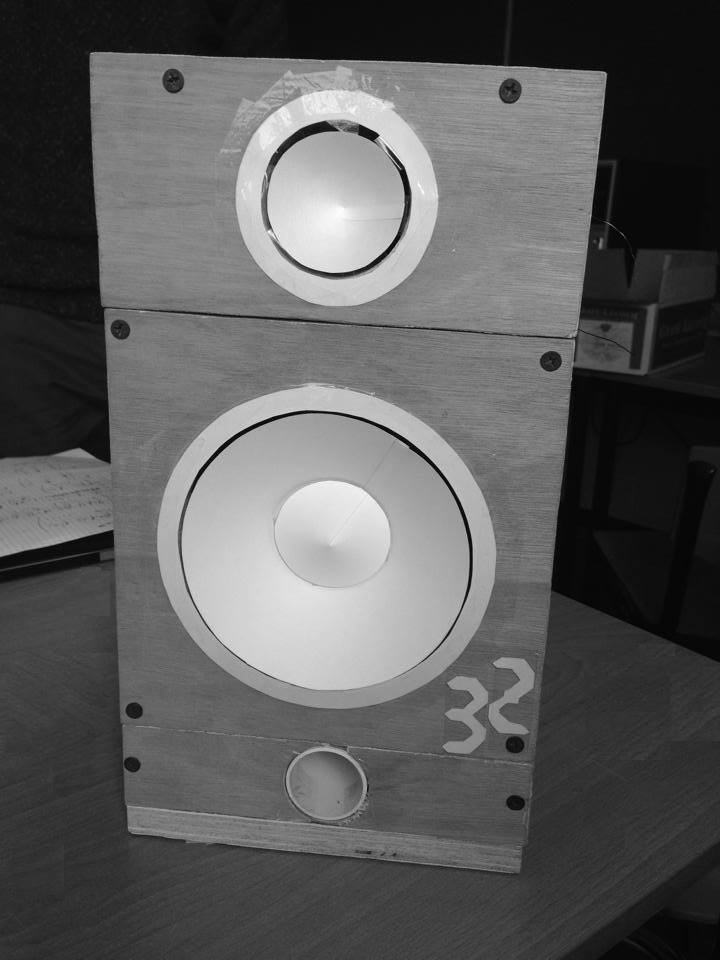
\includegraphics[scale=0.5]{img/PhotoHP} 
\end{center}
\caption{Rendu final des Hauts-Parleurs}		
\label{fig:PhotoHP}		
\end{figure}
\section{Spécifications}

\begin{tabular}{|p{2cm}|p{1.5cm}|p{13.2cm}|}

 \hline 
 \bsc{Groupe 11.32} & \multicolumn{2}{r|} {Date : 12/03/2014}\\
  &  \multicolumn{2}{r|}{Version : 4} \\
 \hline 
	 \multicolumn{3}{|l|}{}\\
	 \multicolumn{3}{|l|}{}\\
	 	\multicolumn{3}{|c|}{\Large{\textbf{Cahier des Charges d'un haut-parleur}}}\\
	\multicolumn{3}{|l|}{}\\
	
 		\multicolumn{3}{|p{16.5cm}|}{\large{\textbf{Contexte :} Dans le cadre du cours de projet, il nous a été demandé de modéliser, construire, faire fonctionner et effectuer des tests sur un haut-parleur pouvant être relié à un smartphone. }}\\
	\multicolumn{3}{|l|}{}\\
 \hline
 
 		\textbf{Date} & \textbf{Origine} & \\
 \hline
 	& &\\
		& & \textbf{Fonctions Principales} \\
 	& &\\
		05-02-2014 & client & \textbf{FP 1 :} Le haut-parleur est capable d’amplifier un signal électrique provenant d’un Smartphone ou d’un baladeur MP3.\\
	& &\\
		05-02-2014 & client & \textbf{FP 2 :} Le haut-parleur est en mesure de transformer un signal électrique en un signal sonore afin de le reproduire fidèlement.  \\
	& &\\
		05-02-2014 & client & \textbf{FP 3 :} Le volume du son est réglable.\\
	& &\\
		05-02-2014 & client & \textbf{FP 4 :} Le signal sonore est réglable en aigus et en graves.\\
	& &\\
		05-02-2014 & client & \textbf{FP 5 :} La puissance maximale du haut-parleur est de $2,5  \watt$.\\
	& &\\
\hline
	 & &\\
	 	& & \textbf{Critères et niveaux des Fonctions Principales} \\
	 & &\\
	 	12-03-2014 & groupe & \textbf{C 1.1} : La fréquence maximale peut être réglée entre $340$ Hz et $6800$ Hz et la fréquence minimale entre $34$ Hz et $340$ Hz.\\
	 & &\\
\hline
	 & &\\
	 & & \textbf{ Fonctions de Contraintes}\\
	 & &\\
		05-02-2014 & client & \textbf{FC 4 :} La prise d’entrée est définie.\\
	 & &\\
		05-02-2014 & groupe & \textbf{FC 5 :} La température de fonctionnement est prédéfinie.\\
	 & &\\
		05-02-2014 & client & \textbf{FC 6 :} Le type d’alimentation du haut-parleur est imposé.\\
	 & &\\
\hline
	& &\\
		& & \textbf{ Critères et niveaux des Fonctions de Contraintes}\\
	& &\\
	 	05-02-2014 & client & \textbf{C 4.1 :} Le signal entre via une prise Jack TRS $3.5$ mm.\\
	& &\\
		05-02-2014 & groupe & \textbf{C 5.1 :} Le haut-parleur est opérationnel dans des températures comprises entre $0$ et $40\,\degreecelsius$.\\
	& &\\
		05-02-2014 & groupe & \textbf{C 6.1 :} Le haut-parleur est alimenté par une source de tension continue et réglable de maximum de $30$ \volt.\\
	 & &\\
\hline
 \end{tabular}

\section{Organisation du rapport}

Dans un premier temps, nous vous exposerons les résultats de notre recherche bibliographique. Ceux-ci concernent les différents types de membranes, de filtres et de caissons. La démarche, les traces ainsi que les sources bibliographiques se trouvent en annexe.

Ensuite, nous entrerons dans le vif du sujet avec le fonctionnement du haut-parleur. Chacun des différents blocs du système, sera décortiqué. Nous vous présenterons leur fonctionnement, leur dimensionnement, la ou les différente(s) méthode(s) pour y arriver ainsi que nos calculs. Nous compareront également les résultats obtenus dans la pratique avec les résultats théoriques. Certains de nos raisonnement, les codes ainsi que les résultats du problème mathématiques se trouvent en annexe.

Enfin, en guise de conclusion, nous ferons le bilan du fonctionnement de notre haut-parleur et essayerons de voir les points où il peut encore être amélioré. Nous réaliserons également le bilan de notre travail de groupe en vous exposants les outils utilisés, nos points forts et nos points faibles.
\section{Description du système}

\begin{figure}
\begin{center}
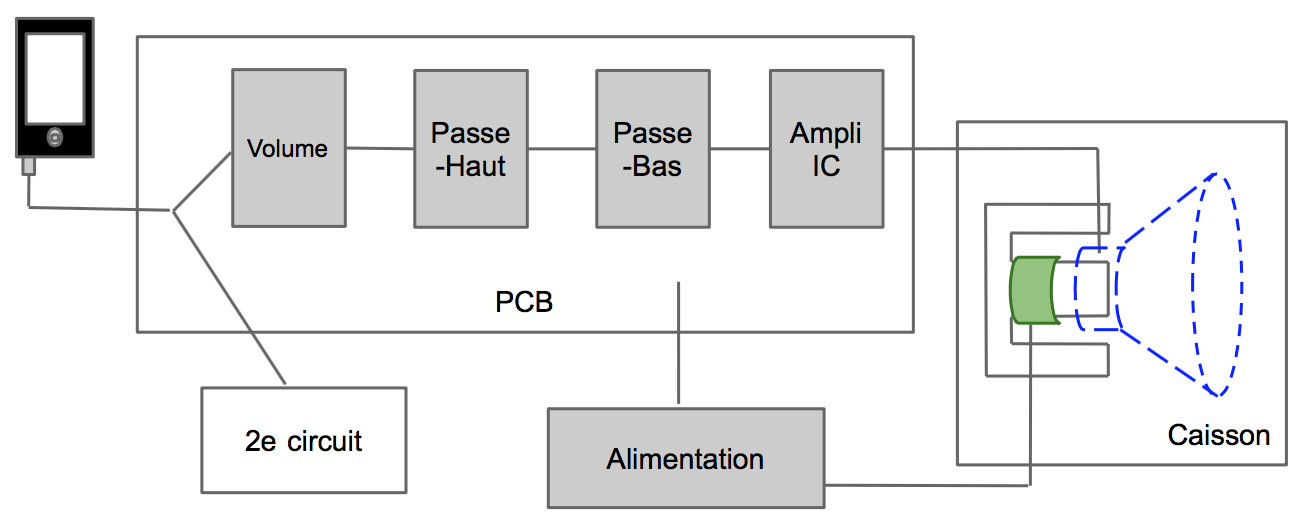
\includegraphics[width=\textwidth]{img/schemacomplet} 
\end{center}
\caption{Schéma général du système}		
\label{fig:schemacomplet}		
\end{figure}

Le système (voir figure~\ref{fig:schemacomplet}) est constitué de 2 parties principales : le circuit imprimé (PCB) et le caisson. 
Ces 2 parties ont été réalisées en double afin de pouvoir gérer un signal stéréo ou d'utiliser un des 2 baffles principalement pour les aigus et l'autre pour les basses. Le circuit de ces 2 hauts-parleurs est identique.
Le signal provenant du smartphone ou baladeur audio est transmis à la PCB grâce à une prise Jack.
La PCB est composée de 4 parties principales :
\begin{itemize}
\item Un récepteur, permettant le branchement du cable jack et permettant d'envoyer un des 2 signaux vers le seconde circuit imprimé.
\item Un potentiomètre, permettant le réglage du volume.
\item Un filtre passe-haut et un filtre passe-bas, permettants respectivement de limiter les basses et les aigus. Ces 2 filtres sont alimentés en +15\,\volt \, et -15\,\volt \, par une source de tension.
\item Un amplificateur, permettant d'amplifier 50 fois le signal de sortie.
\end{itemize}
Le signal à la sortie de la PCB est envoyée vers le caisson et en réalité vers la bobine mobile.
Le caisson peut se décomposer en 3 parties :
\begin{itemize}
\item L'électroaimant, permettant de créer un champ magnétique et donc de faire bouger la bobine mobile. Elle est alimentée par une source de tension de laboratoire.
\item La bobine mobile, permettant de faire vibrer la membrane.
\item La membrane, qui par son mouvement reproduit le son souhaité.
\end{itemize}
Les 2 caissons sont pour leur part différents, un des 2 à plutôt été conçu pour les aigus, il s'agit d'un petit haut-parleur de type ouvert. Le second à été conçu pour les basses, il s'agit d'un plus gros haut-parleur de type bass-reflex.

\chapter{Synthèse des recherches}

\label{Synthèse des recherches}

\section{Membranes}

La séance d’information sur la recherche documentaire en S2
nous a aidé à déterminer les critères pouvant influencer
le bon fonctionnement de notre haut-parleur.
Parmi ceux-là, le choix de la membrane, qui constitue, avec la bobine mobile, la partie mobile
du haut-parleur.


\textbf{large{ICI rajouter la fonction/fonctionnement d'une membrane en qqs mots} et en profiter pour rajouter une référence}


La membrane est un composant complexe dépendant de nombreux paramètres. Le choix de sa forme, sa dimension et son matériau ainsi que son bon maintient ont une grande influence sur le rendu sonore. Un choix judicieux de ces critères permet d'optimiser le rendu sonore dans les aigus, les médiums ou les graves, selon ses désirs.

Tout d’abord, la membrane d’un haut-parleur artisanal
se doit d’être légère en masse et relativement rigide
car cela permet un déplacement plus facile et
sans risque d’endommager l’ensemble.
Le papier est donc, surprenamment, un matériau de choix.

Ensuite, la plupart des études faites jusqu’à ce jour,
ont montré que les membranes en forme de cône
donnent le son le plus puissant et de la meilleure qualité.

En effet, la membrane devant être légère, une forme plane entraînera une diminution du volume d’air à déplacer et par conséquent un rendement faible.~\footnote{Extrait du brevet \textit{\og Compound Loudspeaker Diaphragm (US3153463 A)\fg} de Novak James F. \cite{f1964compound}}

%Preuve en est que cette forme est utilisé dans la quasi-totalité
des haut-parleurs sur le marché.
En particulier, la membrane devant être légère,
une forme non circulaire entrainera souvent des déformations non désirées,
diminuant ainsi le rendement sonore et, à terme, abîmera la membrane.
%
Le diamètre et la profondeur du cône de ces membranes
ont aussi un impact sur la bande de fréquences
qu’elles sont capables de reproduire fidèlement.
En effet, un cône possédant un petit diamètre ainsi qu'une petite profondeur
permet une meilleure réponse aux hautes fréquences,
tandis que ceux ayant un diamètre plus grand et et très profonds sont plus adaptés aux bases et moyennes fréquences.~\footnote{Extrait de Ryan Miller, \og Modal Analysis of Loudspeaker Diaphragms\fg p. 2}
Pour cette raison, nous avons choisi de donner un diamètre
différent aux membranes de nos deux haut-parleurs,
utilisés pour isoler les graves et médiums dans un cas,
et les aigus dans l'autre.

Enfin, afin de reproduire des sons le plus fidèlement possible, il est important que la partie mobile du haut-parleur bouge de manière axiale par rapport au noyau.
Deux dispositifs sont prévus à cet effet \cite[p.~6486]{Larousse} : 
\begin{itemize}
\item un dispositif de centrage de la bobine mobile ou \textit{spider} qui \begin{quote} a pour but d’empêcher la bobine mobile d’entrer en contact avec les parois de l’entrefer, sans toutefois gêner les mouvements utiles. Le spider idéal doit s’opposer à tout mouvement latéral de la bobine mobile ; il doit au repos la maintenir au centre de la zone de champ magnétique uniforme, ne pas exercer une résistance au mouvement augmentant avec l’amplitude et ne pas avoir de résonance propre~\footnote{Extrait de J.B., \og La Grande Encyclopédie Larousse [en ligne]\fg : \url{http://www.larousse.fr/archives/grande-encyclopedie/page/6486}}.\end{quote}
\item un dispositif de centrage et de suspension de la membrane, qui sert de raccord entre le saladier et la membrane. Il doit être le plus flexible possible, pour ne pas gêner le mouvement de la membrane.
\end{itemize}







\section{Caissons}

\textbf{\textsc{À reformuler}}

Il existe sur le marché des haut-parleurs
différents types de caisson, tels que
les caisson basse-reflex, les caisson clos et encore bien d’autres.

Dans le choix du caisson de notre haut-parleur,
nous avons opté pour le caisson basse-reflex pour les graves
et un caisson ouvert pour les aigus.
Le premier s’explique par le fait que le caisson basse-reflex
contrairement à d’autres tel que celui clos permet de récupérer
une partie des ondes se trouvant à l’arrière.
Avec ce système, lorsque les ondes situées a l’arrière sont en phase
avec celles émises a l’avant du haut- parleur, elle les amplifie,
tandis que lorsqu’elles  sont opposées,
ces ondes sont renvoyées à l’extérieure afin de réduire la résonance.
Cependant, ce système a pour inconvénient de provoquer dans certains cas
des bruits sonores dans l’évent, situe dans la partie inferieur du caisson.
En ce qui concerne le caisson ouvert,
le court-circuit acoustique ayant pour conséquence la perte du niveau
en dessous d’une certaine fréquence,
nous avons opté pour celui-ci qui réduit cet effet.


\chapter{Signal d'entrée et réglage de volume}

\begin{center}
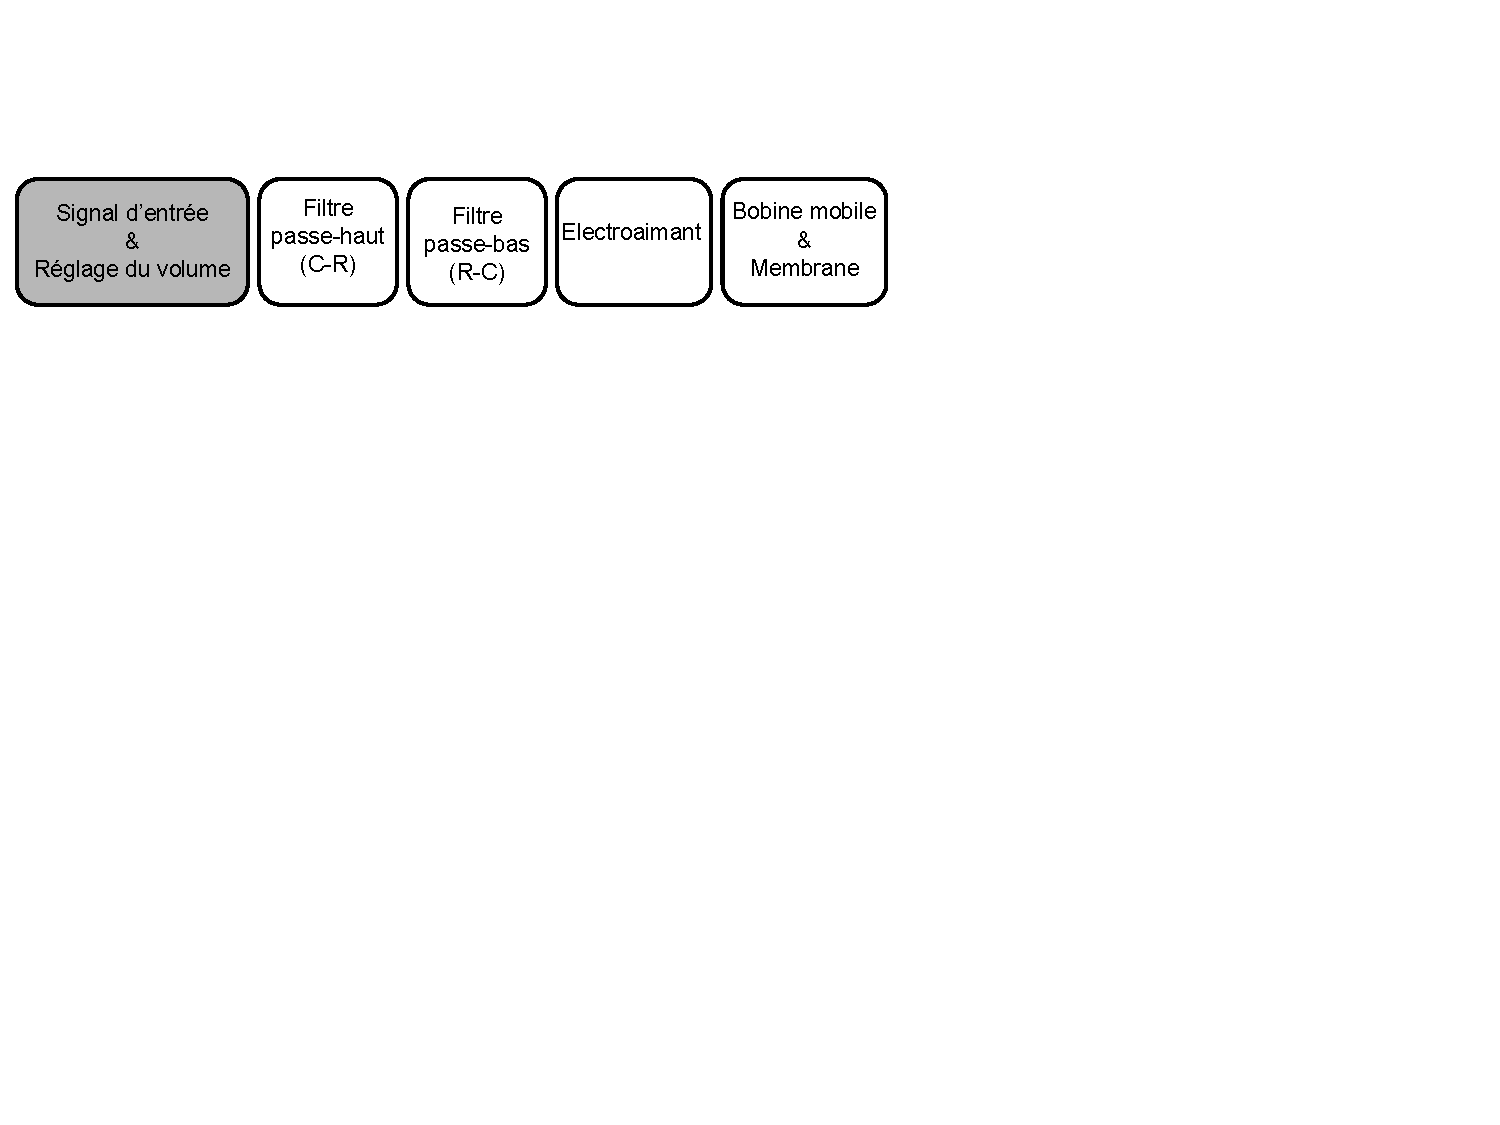
\includegraphics[width=\textwidth]{img/Schemabloc1}
\end{center}

\section{Introduction}
La sortie typique d'un smartphone à plein volume est une différence de potentiel de $\milli\volt$ . Cela peut paraitre peu, 
mais une telle amplitude peut être dangereuse pour les puces électroniques du circuit si elle n'est pas diminuée par
un dispositif quelconque. De plus, pouvoir faire varier l'amplitude permet de faire varier le volume de manière
indépendante par rapport au smartphone.
\section{Résolution}
Pour répondre à ces deux attentes, il nous suffit de réaliser un diviseur de tension réglable, que nous avons réalisé 
à l'aide d'un potentiomètre à l'entrée de la plaquette électronique. Le schéma ci dessous illustre la situation. Le potentiomètre 
à été schématisé en 2 résistances simples.

\begin{figure}[h!]	
\begin{center}
\begin{circuitikz} \draw
 (1,2)
  to[R,v=$v_1$, l=$R_1$, *-*] (1,0)
 (1,2) to[short, *-o] (0,2)
  node[anchor=east]{A}
 (1,0) to [R,v=$v_2$, l=$R_2$] (1,-2)
 (1,0) to[short, *-o] (3,0)
node[anchor=west]{B}
 (1,-2)node[ground]{}
;\end{circuitikz}
\end{center}
\caption{Potentiomètre}		
\label{potentiometre}		
\end{figure}

La différence de tension $V =  v_1 + v_2$ est la différence de potentiel provenant du smartphone. 
En utilisant la loi d'ohm, nous obtenons $V = I (R_1 + R_2)$ et $v_2 = I R_2$. Puisque $I = \frac{V}{R_1+R_2}$, nous obtenons 
$v_2 = \frac{V R_2}{R_1+R_2}$. $R_1+R_2$ est la résistance totale du potentiomètre, $R_1$ et $R_2$ sont inversément proportionnelles. Plus $R_2$ 
sera grande et donc proche de la résistance totale du potentiomètre, plus la tension en $B$ sera proche de la tension fournie en $A$. Nous voyons 
donc bien qu'en faisant varier le sélecteur du potentiomètre, nous faisons varier la tension en $B$, ce qui fera varier le volume du 
haut-parleur.
\chapter{Filtres de fréquences}

\subsection*{Introduction}

Les filtres servent à limiter les fréquences transmises au haut-parleur
à un certain intervalle, réglable par des potentiomètres.
Dans le schéma général du circuit (Fig.~\ref{fig:schema-gen-filtres}),
ils se situent après le réglage de volume, et avant l'amplification du signal.

Ces deux filtres (passe-haut et passe-bas) sont les éléments les plus complexes
du circuit, et ils ont constitué
une partie importante du travail de modélisation que nous avons effectué.
Nous y consacrons d'ailleurs trois annexes:
\begin{itemize}
    \item D'abord, une découverte de la méthode des phaseurs
        comme un isomorphisme
        entre les fonctions sinusoïdale et les complexes
        (Annexe~\ref{chap:phaseurs}).
    \item Ensuite,
        l'identification linéaire par morceaux du gain des filtres utilisés
        (Annexe~\ref{chap:approx-lin}).
    \item Enfin,
        une réflexion sur l'origine de ces tendances linéaires et
        la généralisation de leur identification à d'autres types de filtres
        (Annexe~\ref{chap:filtres-gen}).
\end{itemize}

Dans ce chapitre,
nous nous concentrerons plutôt sur le rôle pratique de ces filtres
dans notre circuit.

\subsubsection*{Plan du chapitre}
\begin{enumerate}
    \item Nous commencerons par expliquer plus en profondeur la \emph{fonction}
        des deux filtres de fréquence et leur effet dans la perception du son.
    \item Puis nous présenterons leurs \emph{caractéristiques techniques},
        c'est-à-dire les composants impliqués et leur agencement.
    \item Ensuite, nous ferons la \emph{modélisation} mathématique
        des deux filtres
        par la méthode des phaseurs et nous donnerons une interprétation
		des résultats obtenus.
    \item Après cela, nous justifierons le \emph{dimensionnement} par rapport
        aux fréquences de coupure.
    \item Enfin, nous ferons la synthèse des mesures effectuées ainsi qu'une
        \emph{confrontation} entre la théorie et la pratique.
\end{enumerate}

\section{Fonction}

Comme expliqué dans l'introduction, les filtres servent à limiter
le domaine de fréquences du signal à un certain intervalle
$[f\ind{min},f\ind{max}]$.
Les fréquences situées en-dehors de cet intervalle seront atténuées,
comme l'illustre la figure~\ref{fig:filtre-ideal} en échelle log-log.

Ce genre de dispositif s'appelle un filtre \emph{passe-bande},
car il tend à laisser passer une bande de fréquences et exclure le reste.
Dans notre cas, il est formé par la combinaison d'un filtre
\emph{passe-haut} et d'un filtre \emph{passe-bas}.

Le filtre \emph{passe-haut} laisse passer les hautes fréquences,
il se charge donc d'atténuer les basses fréquences ($f<f\ind{min}$);
tandis que le filtre \emph{passe-bas} laisse passer les basses fréquences,
il se charge donc d'atténuer les hautes fréquences ($f>f\ind{max}$).

L'oreille humaine est capable de

\section{Caractéristiques techniques}

Comme illustré dans la figure~\ref{schema-elec-filtres},
la sous-ensemble des filtres est composé, dans l'ordre, de:
\begin{enumerate}
    \item un premier suiveur répétant le signal venant du réglage de volume
        à travers le JP\,1, grâce à l'ampli op LM358N;
    \item le filtre passe-haut formé d'un
        condensateur de capacité $C_2 = 470\,\nano\farad$;
        et un potentiomètre de résistance
        maximale $R\ind{2,max} = 1\,\kilo\ohm$;
    \item un deuxième suiveur, sur le même ampli;
    \item le filtre passe-bas formé d'un potentiomètre de résistance
        maximale $R\ind{3,max} = 10\,\kilo\ohm$
        et un condensateur de même capacité $C_3 = 470\,\nano\farad$;
    \item la sortie au niveau du JP\,2 vers l'amplificateur audio.
\end{enumerate}

%Référencer ici les datasheets.

L'ampli op et les capacités nous étaient imposés,
et pour le reste, nous discuterons le choix des potentiomètres dans
la section~\ref{dimen-filtres} sur le dimensiomment.

\section{Modélisation}

Dans cette section, nous allons commencer par analyser les filtres
par une bonne intuition,
ensuite nous poserons nos hypothèses de modélisation,
puis nous trouverons les fonctions de transfert et en extrairons
des tendances générales
et les expressions des gains et amplitudes,
et enfin nous interpréterons les résultats.

\subsection{Intuition}

Le filtre passe-haut comme le filtre passe-bas
consistent en une capacité et une résistance en série,
avec un signal imposé à leurs bouts.
La tension de sortie est prise aux bornes de la résistance pour le passe-haut
et aux bornes de la capacité pour le passe-bas.

On peut voir la capacité comme un réservoir qui se charge lentement avec le
courant augmenter la tension, tandis que la résistance est un dispositif
qui laisse passer le courant, mais en freinant par une différence de tension.

Pour de petites fréquences, la tension d'entrée bouge lentement.
La capacité a donc tout le temps de charger,
s'approchant à tout moment de la tension d'entrée,
avec un courant très faible.
Autrement dit, elle agit comme un circuit ouvert.
La résistance, par conséquent, n'a pas une grande différence
de tension à ses bornes.

Pour de hautes fréquences, au contraire, la tension d'entrée bouge rapidement.
La capacité n'a donc pas du tout le temps de charger,
et la différence de tension à ses bornes est très faible,
pour n'importe quel courant.
Autrement dit, elle agit comme un court-circuit.
La résistance, par conséquent, aura à ses bornes
une différence de tension qui s'approche de la tension d'entrée.

En conclusion, on s'attend à ce que le filtre passe-haut,
qui prend la tension aux bornes de la résistance,
atténue les petites fréquences et conserve les hautes fréquences;
et à ce que le filtre passe-bas,
qui prend la tension aux bornes de la capacité,
conserve les petites fréquences et atténue les hautes fréquences.
Fort heureusement, cela respecte leurs définitions.

\subsection{Hypothèses}

Pour modéliser la réponse des filtres à différents signaux nous allons utiliser
la méthode des phaseurs, comme décrite dans l'annexe~\ref{chap:phaseurs}.
Nous supposerons donc ici que le signal est une sinusoïde pure, les autres cas
pouvant s'y ramener en prenant la transformée de Fourier.

Nous supposons également que tous les composants et les liaisons entre ceux-ci
sont idéaux.
En particulier, nous considérons que les courants d'entrée de l'ampli-op
et l'ampli audio sont négligeable.

\subsection{Résolution}

Définissons comme sur la figure~\ref{fig:filtres-v1v2v3}
$v_1(t),v_2(t),v_3(t)$ les tensions
à l'entrée, après le filtre passe-haut et après le filtre passe-bas;
et $\overline{V_1}, \overline{V_2}, \overline{V_3}$ leurs phaseurs associés.

Tout le courant passant à travers le condensateur $C_2$ passe
aussi à travers la résistance $R_2$.
Par conséquent, on peut appliquer la loi de division des tensions,
avec les impédances $\frac{1}{j\omega C_2}$ et $R_2$:
\begin{equation}
    \overline{V_2} = \frac{R_2}{\frac{1}{j\omega C_2} + R_2}\,\overline{V_1}
    = \frac{j\omega R_2C_2}{1+j\omega R_2C_2}\,\overline{V_1}
\end{equation}
La fonction de transfert du filtre passe-haut est donc
$H\ind{ph}(j\omega) = \frac{j\omega R_2C_2}{1+j\omega R_2C_2}$.

Pour le filtre passe-bas, on peut supposer de manière similaire que
le courant à l'entrée de l'ampli audio est négligeable,
et appliquer la loi de division des tensions avec les impédances
$R_3$ et $\frac{1}{j\omega C_3}$:
\begin{equation}
    \overline{V_3} =
    \frac{\frac{1}{j\omega C_3}}{\frac{1}{j\omega C_3} + R_3}\,\overline{V_2}
    = \frac{1}{1+j\omega R_3C_3}\,\overline{V_2}
\end{equation}
Le gain en tension du filtre passe-bas est donc
$H\ind{pb}(j\omega) = \frac{1}{1 + j\omega R_3C_3}$.

Étant donné que la tension $v_2$ est répétée de la sortie du filtre passe-haut
à l'entrée du filtre passe-bas, la fonction de transfert totale du système est:
\begin{align}
    H\ind{tot}(j\omega) &= H\ind{ph}(j\omega)\,H\ind{pb}(j\omega) =
    \frac{j\omega R_2C_2}{1 + j\omega R_2C_2}\,\cdot\,
    \frac{1}{1 + j\omega R_3C_3}\\
    &= \frac{j\omega R_2C_2}{1 + j\omega\,(R_2C_2+R_3C_3) +
        (j\omega)^2\,(R_2C_2R_3C_3)}
\end{align}

\subsection{Tendances}

\textbf{\textsc{À bouger en annexe}}

Avant de calculer les gains et déphasages en détail,
nous allons mettre en évidence des tendances dans les fonctions de transfert.

Commençons par le filtre passe-haut, dont la fonction de transfert est
$H\ind{ph}(j\omega) = \frac{j\omega R_2C_2}{1+j\omega R_2C_2}$.
Le dénominateur contient deux termes qui «dominent» à tour de rôle:
le premier, 1, sera le plus grand en norme pour de petites valeurs de $\omega$,
jusqu'au point $\omega = 1/R_2C_2$, où $j\omega R_2C_2$, qui grandit
avec $\omega$, «prendra le relais».
Notons cette pulsation critique $\omega\ind{bas}= 1/R_2C_2$ et
appelons-la \emph{pulsation de coupure}.

Plus précisément,
\begin{itemize}
    \item quand $\omega << \omega\ind{bas}$,
        $H\ind{ph} \approx \frac{j\omega R_2C_2}{1} = j\omega R_2C_2$;
    \item quand $\omega >> \omega\ind{bas}$,
        $H\ind{ph} \approx \frac{j\omega R_2C_2}{j\omega R_2C_2} = 1$.
\end{itemize}

Cette rapide analyse confirme notre intuition et la précise:
\begin{itemize}
    \item pour de petites pulsations,
        le signal est de moins en moins atténué et est en avance de $\pi/2$
        sur l'entrée (à cause du facteur $j$);
    \item à partir de la pulsation de coupure le signal sera presque
        restitué à l'identique.
\end{itemize}

Pour le filtre passe-bas, la situation est analogue.
Le dénominateur fait apparaître une pulsation de coupure
$\omega\ind{haut} = 1/R_3C_3$.
À partir de la fonction de transfert
$H\ind{pb}(j\omega) = \frac{1}{1 + j\omega R_3C_3}$,
on découvre que:
\begin{itemize}
    \item quand $\omega << \omega\ind{haut}$, $H\ind{pb} \approx 1$;
    \item quand $\omega >> \omega\ind{haut}$, $H\ind{pb}
        \approx \frac{1}{j\omega R_3C_3}$;
\end{itemize}
ce qui confirme et précise notre intuition:
\begin{itemize}
    \item pour de petites pulsations, le signal sera presque restitué
        à l'identique;
    \item à partir de la pulsation de coupure, le signal est de plus en plus
        atténué
        et est en retard de $\pi/2$ sur l'entrée (à cause du facteur $1/j$).
\end{itemize}

\subsection{Gain et déphasage}

Intéressons-nous maintenant de manière plus rigoureuse
au \emph{gain} (rapport d'amplitude) et au  \emph{déphasage} (décalage)
entre l'entrée et la sortie.
Ils correspondent respectivement au module et à l'argument de la fonction de
transfert.

C'est-à-dire, pour le filtre passe-haut:
\begin{align}
    G\ind{ph}(j\omega) &= |H\ind{ph}(j\omega)|
    = \frac{|j\omega R_2C_2|}{|1 + j\omega R_2C_2|}
    = \frac{\omega R_2C_2}{\sqrt{1+(\omega R_2C_2)^2}}\\
    \phi\ind{ph}(j\omega) &= \arg\big(H\ind{ph}(j\omega)\big)
    %= \arctan(j\omega R_2C_2) - \arctan(1+j\omega R_2C_2)
    = \arctan\left(\frac{1}{\omega R_2C_2}\right)
\end{align}
et pour le filtre passe-bas:
\begin{align}
    G\ind{pb}(j\omega) &= |H\ind{pb}(j\omega)|
    = \frac{|1|}{|1 + j\omega R_3C_3|}
    = \frac{1}{\sqrt{1+(\omega R_3C_3)^2}}\\
    \phi\ind{pb}(j\omega) &= \arg\big(H\ind{pb}(j\omega)\big)
    = \arctan(-\omega R_3C_3)
\end{align}

Ces résultats sont illustrés par des graphes dans
les figures~\ref{fig:graphes-pb} et~\ref{fig:graphes-pb}, avec en abcisse la pulsation
et en ordonnée le gain et le déphasage.
Les tendances découvertes sont en pointillés.
Ici, les potentiomètres sont tous deux réglés à $20\%$,
donc $R_2 = 200\,\ohm$ et $R_3 = 2\,\kilo\ohm$.

Nous utilisons une échelle logarithmique pour les fréquences
ou pulsations, ainsi que pour les gains.
Les raisons de ce choix sont expliquées en détail dans
la section~\ref{sec:log}.

Enfin, pour la combinaison des deux filtres,
les fonctions de transfert sont multipliées,
donc les gains sont multipliés et les déphasages sont additionnés.
Le résultat est illustré dans la figure~\ref{fig:graphes-bande}.

\subsection{Interprétation}

\textbf{\textsc{À réécrire et compléter}}

Nous pouvons voir dans la figure~\ref{fig:graphes-bande}
que notre combinaison de filtres a bien le résultat attendu.
En effet, on voit que les signaux dont les pulsations sont dans l'intervalle
$[\omega\ind{bas},\omega\ind{haut}]$
\footnote{Ou dont les fréquences sont dans l'intervalle
    $[f\ind{bas},f\ind{haut}]$ avec
    $f\ind{bas} = \omega\ind{bas}/2\pi$ et
    $f\ind{haut} = \omega\ind{haut}/2\pi$.}
sont conservées.

La première remarque à faire est que les filtres ne sont pas des filtres idéaux
en ce sens que la coupure de signal n'est pas brutale:
dans le filtre passe-haut comme dans le filtre passe-bas,
l'amplitude décroit linéairement en échelle log-log.
Cela dit, ce n'est pas forcément une mauvaise chose.
En effet, cela permet d'atténuer certaines fréquences sans pour autant
les supprimer complètement.


\chapter{Electro-aimant}
\section{Introduction}
Dans la quasi totalité des haut-parleurs d'aujourd'hui se trouve un aimant permanent générant un champ magnétique.
N'ayant pas de tel aimant à disposition, nous avons réalisé un électro-aimant grâce à du fil de cuivre enroulé autour 
d'un coeur en forme de E de fer orienté, matériau ferromagnétique.
\section{Intuition}
Le solénoide étant enroulé sur un coeur magnétique, et l'entrefer étant petit, le champ magnétisant dans 
une boucle passant par le coeur du solénoide, l'entrefer et revenant au solénoide à travers une branche 
du E doit être constant. Ceci pourrait être un bon point de départ pour obtenir le champ $B$ présent dans l'entrefer.
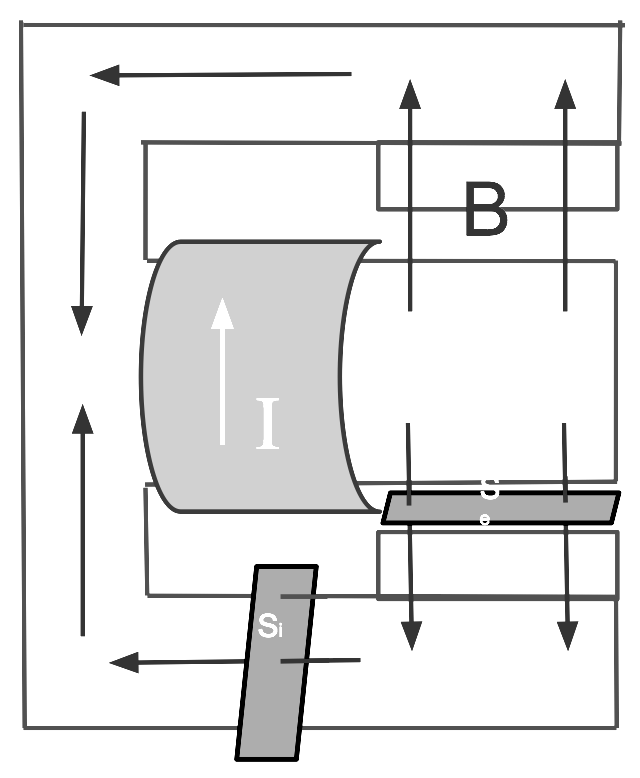
\includegraphics{img/schema-aimant-bobine}
\section{Hypothèses}
\begin{itemize}
\item Le solénoide étant enroulé autour d'un coeur ferromagnétique ayant \[\mu = \mu_0 * 1600\], et puisque les 
tours du solénoides sont fortements serrés et une épaisse bobine, nous supposons qu'aucun champ ne passe 
à entre les fils et que tout le champ magnétique généré passe par l'entrefer.\\
\item Nous supposons également que tout le champ magnétisant $H$ passe directement par l'entrefer, et que rien ne passe par 
le dessus ou le dessous de la branche intermédiaire du E.
\item Le champ $B$ que nous voulons obtenir dans l'entrefer est un champ de $0,1\tesla$. Cette valeur fut choisie car elle nous 
d'obtenir une force suffisante pour faire bouger la membrane avec une amplitude satisfaisante tout en gardant la bobine 
mobile relativement légère car avec peu de tours de fils de cuivre.
\end{itemize}
Il est à noter que notre entrefer mesure $0.5\centi\meter$ car nous avons rajouter des plaquettes afin de le réduire.
\section{Développement théorique}
Le champ magnétisant généré par la bobine est 
$\int{H dl} = N I$
En prenant une boucle dans notre circuit magnétique, grâce à Gauss généralisée, nous avons que
$H_i l + H_e e = N I (1)$
Nous avons également que $B_i S_i = B_e S_e (2)$  avec $S_i \simeq S_e$
ainsi que \\
$B_i = \mu H_i \:et\:  B_e = \mu_0 H_e$
Puisque \[\mu \gg \mu_0\]nous savons que $H_i \ll H_e$ grâce à l'équation (2).
Nous pouvons alors réécrire l'équation (1) $H_e = \frac{N I}{e}$.
Nous obtenons alors le champ $B$ recherché $B = B_e = \mu_0 \frac{N I}{e}$.
\section{Calcul}
Puisque nous voulons obtenir un champ $B = 0,1 \tesla$, et que nous fournissons $I = 1 A$ afin de ne pas faire trop 
chauffer la bobine, et que nous connaissons $e$, nous pouvons calculer le nombre de tours $N$ requis pour obtenir 0.1\tesla.
$N = \frac{0.1 * 0.5}{\mu_0 * 1} = 400$
\section{Résultats pratiques}
Grâce à un tesla-mètre, nous avons pu vérifier que notre première hypothèse était correcte, car nous n'obtenions 
qu'environ $10 \milli\tesla$ à côté de la bobine. 
\\La deuxième hypothèse était cependant trop forte par rapport à la réalité, car une 
partie du champ magnétique passe en dehors de l'entrefer. Afin de palier à ce déficit, nous avons exagéré le nombre de 
tours de la bobine mobile ($N \simeq 550$) et nous avons alors obtenu $B = 110 \milli\tesla$ dans l'entrefer, 
ce qui était le champ désiré.

\chapter{Bobine mobile et membrane}

\begin{center}
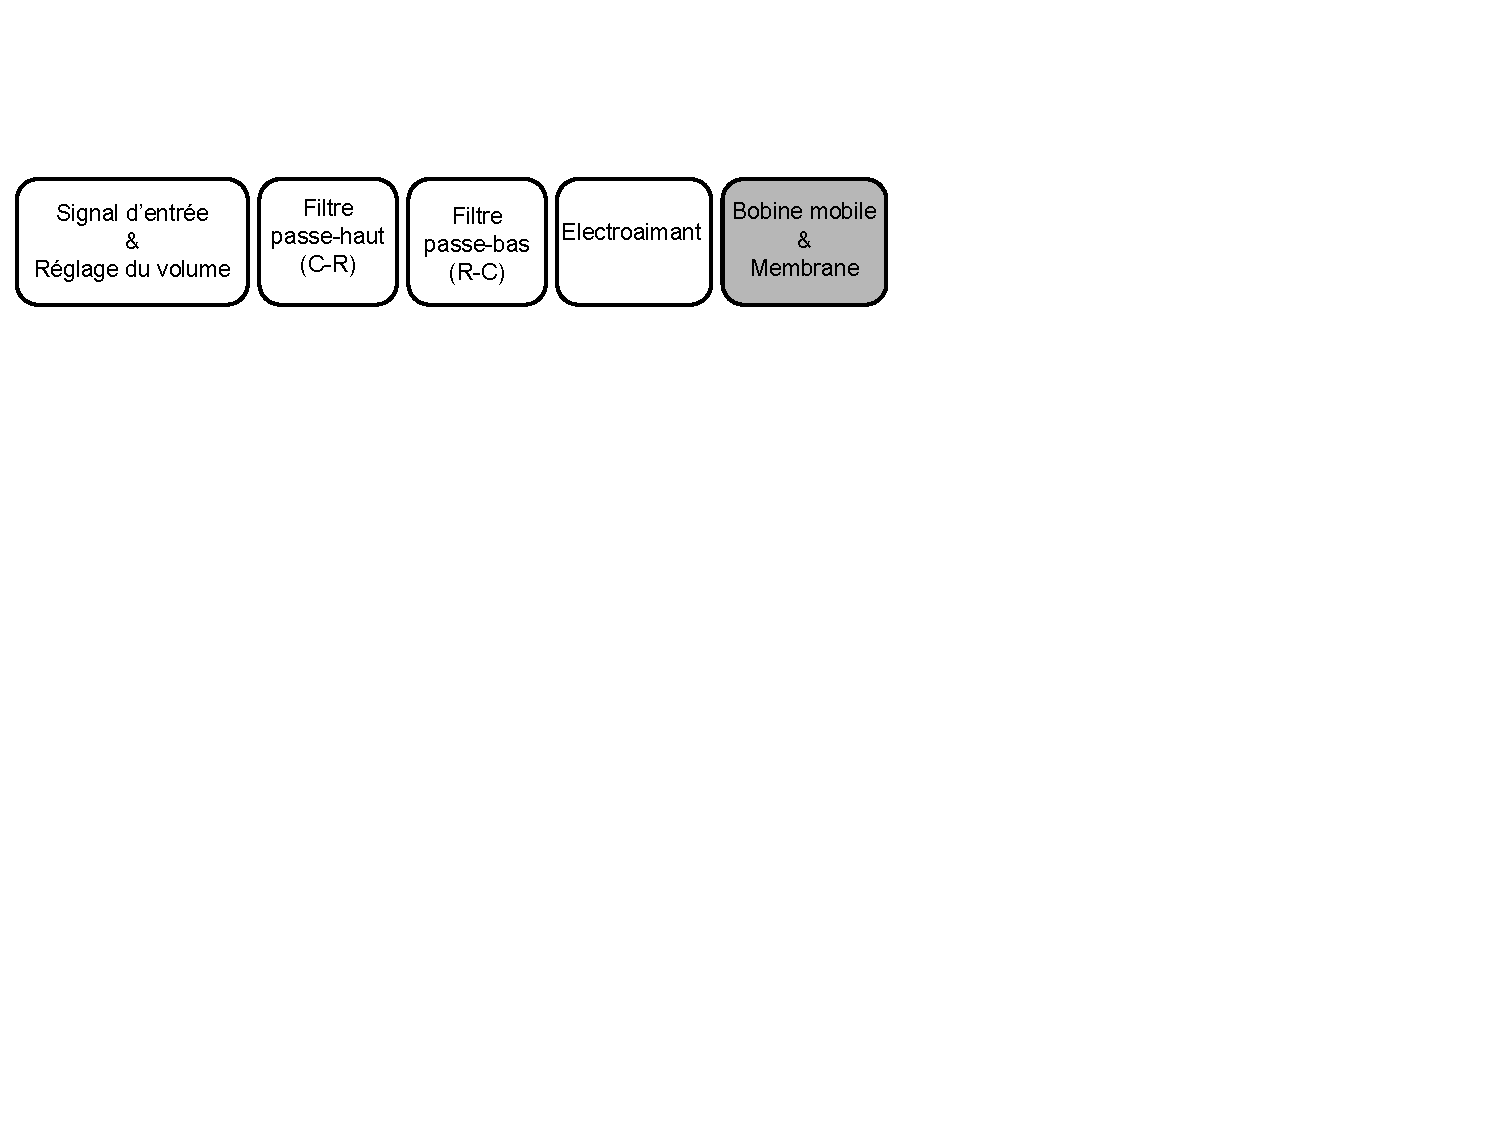
\includegraphics[width=\textwidth]{img/Schemabloc4}
\end{center}

\section{Introduction}
La bobine mobile est reliée à l'output du circuit imprimé et permet de faire bouger la membrane. Elle se situe dans 
l'entrefer. Suivant la direction du courant dans la bobine, direction déterminée par la différence de potentiel
entre les output de la PCB, la force exercée par le champ magnétique sur celle-ci poussera la 
membrane dans un sens ou dans l'autre.

\section{Hypothèses}
Nous utiliserons les valeurs théoriques obtenues durant la partie précédente sur l'électroaimant dans nos calculs.
Ainsi, le champ dans l'entrefer $B = 0.1\tesla$, la hauteur de l'entrefer est $h = 0.01\meter$, sa longueur 
$e = 0.005\,\meter$. Nous supposons également que $B$ est uniforme dans l'entrefer. Enfin, nous avons 
calculé que la longueur de fil perpendiculaire au champ par tour de bobine est de $2h$ .

\section{Modélisation}

\subsection[a]{Bobine mobile}

\begin{figure}	
\begin{center}
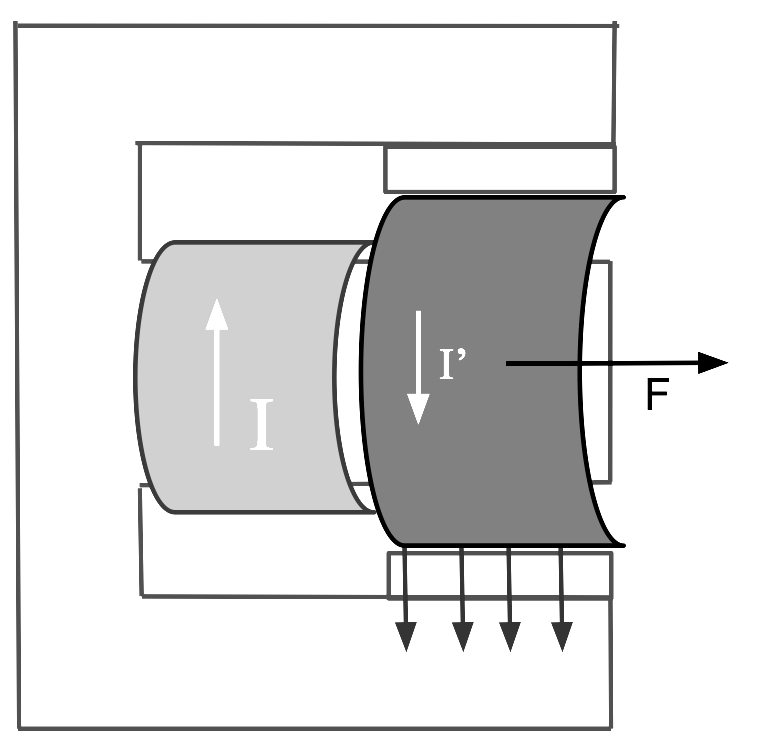
\includegraphics[scale=0.5]{img/bobine-mobile}
\end{center}
\caption{Schema de la bobine mobile}		
\label{fig:bobinemobile}		
\end{figure}

La force exercée par un champ magnétique sur un fil parcouru par un courant est $F =  I' l \times B$\, (Force de Laplace). Puisque 
chaque boucle intercepte $2h$ de longueur de fil perpendiculaire, et que la bobine mobile est faite de $N'$ tours, nous pouvons
donc en déduire que $F_{tot} = 2 h N' I' B$ \. Nous avons $B = \frac{\mu_0 N I}{e}$ qui fut déterminé 
lors du chapitre précédent. La force exercée par le champ magnétique sur la bobine est donc 
$ |F_{tot}| = 2 \mu_0 N N' I I' \frac{h}{e}$ . La direction de la force dépend du sens du courant dans la bobine, et 
celui-ci est déterminé par la différence de potentiel entre les deux output de la plaquette. Selon le courant et son
intensité, la bobine (et donc la membrane liée à celle-ci) sera accélérée dans une direction ou son opposé, reproduisant 
ainsi la bande sonore de la musique.

Si la différence de tension entre les 2 output est de $5\,\volt$, le courant dans la bobine mobile est de 
$I' = \frac{5\,\volt}{8\,\ohm} = 0.625\,\ampere$ ($8\,\ohm$ est la résistance totale de la bobine mobile avec une petite 
résistance ajoutée). La force exercée sur la bobine est donc de $F = 0.04\,\newton$

\subsection[b]{Analyse mécanique de la membrane}
Considérons toutes les forces s'appliquant sur la membrane :
\begin{itemize}
\item La force exercée par l'électro-aimant $ \vec{f} $ 
\item La force de rappel du ressort $ - k \vec{x} $
\item La force due aux dissipations $ - h \dot{\vec{x}} $
\end{itemize}

Cela nous permet d'exprimer l'équation du mouvement :
\begin{equation}
\mathrm{Somme\ des\ forces} = \vec{f} - k \vec{x} - h \dot{\vec{x}} = m \ddot{\vec{x}}
\Leftrightarrow m \ddot{\vec{x}} + k \vec{x} + h \dot{\vec{x}} = \vec{f}
\end{equation}

Ou sous forme phasorielle :
\begin{equation}
m (j\omega)^2 X+ h (j\omega)X + kX = F
\Leftrightarrow X = \frac{F}{k + hj\omega - m {\omega}^2}
\end{equation}

On suppose que les premières couches d’air devant la membrane sont incompressibles. Par conséquent, elles suivent le même déplacement $X$.
Pour les déplacer, il faut une pression $P$ telle que 
\begin{equation}
P\cdot A = m\ind{air} (j \omega)^2X
\Rightarrow P = m\ind{air} (j \omega)^2 \frac{F}{k+hj \omega -m \omega^2}
\end{equation}
La pression, et donc le volume perçu, ont une courbe caractéristique du type :

\begin{figure}[h!]
    \centering
    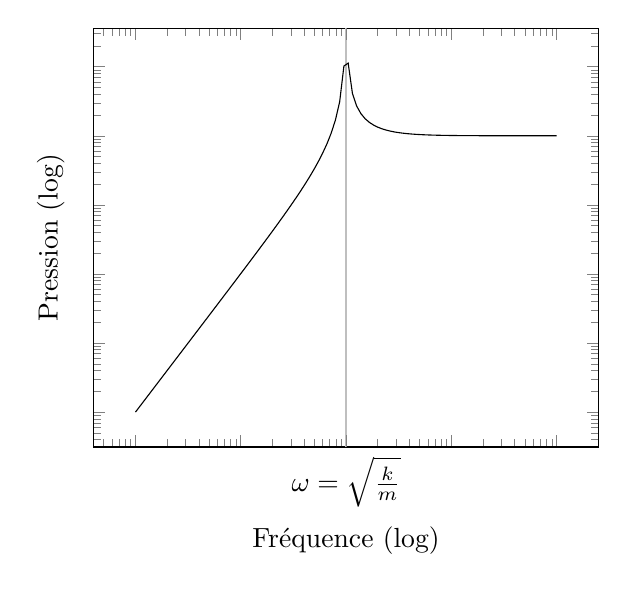
\begin{tikzpicture}
        \begin{loglogaxis}[
                xlabel={Fréquence (log)},
                ylabel={Pression (log)},
                width=8cm,
                xticklabels=\empty,
                yticklabels=\empty,
                extra x ticks={1000},
                extra x tick style={grid=major},
                extra x tick labels={$\omega = \sqrt{\frac{k}{m}}$}
            ]
            \addplot[domain=1e1:1e5,samples=100]
            {x^2/sqrt((1000-x^2/1000)^2+(1e-5*x)^2)};
        \end{loglogaxis}
    \end{tikzpicture}
    \caption{Amplitude de la variation de pression en fonction de la fréquence}
\end{figure}

Il vaut donc mieux minimiser la pulsation critique $\omega = \sqrt{\frac{k}{m}}$ afin d’avoir une réponse égale pour toutes les fréquences.

\section{Confrontation}
Cette force relativement faible fut suffisante pour obtenir une qualité audio acceptable et un volume correct. 
En minimisant la masse de la bobine mobile (seulement 5\,\meter de fil utilisé contre 50 pour l'électro-aimant, 
donnant une masse d'environ 16\,\gram), nous obtenions une grande accélération de $2.5\,\meter\per\second^2$. 

\chapter{Conclusion}

\section{Bilan des réalisations}

Il est maintenant temps de faire le bilan du fonctionnement et des réalisations concernant notre haut-parleur, ainsi que de voir si celui-ci correspond aux spécifications de notre cahier des charges.

Point de vue réalisation techniques, le système final est constitué d'une prise Jack TRS 3,5 mm permettant le transfert d'un signal provenant d'un baladeur de musique ou d'un smartphone vers un circuit électrique. Ce circuit est équipé d'un potentiomètre permettant le réglage en volume, d'un filtre passe-haut et d'un filtre basse-bas permettant le réglage en basses en en aigus. Le champ magnétique est produit par un électro-aimant, alimenté par une source de tension de laboratoire. Le son, quant à lui, est produit grâce à une membrane en papier fixée à une bobine mobile, et reliée au circuit. Un amplificateur intégré au circuit permet d'amplifier 50 fois le signal reçu par le smartphone. Notre haut-parleur est donc conforme aux attentes du Cahier des Charges.

Outre les spécifications du CdC, nous avons décidé, afin d'améliorer le rendu du son, de concevoir deux hauts-parleurs différents. Un petit assurant la fonction de tweeter et un plus grand comme woofer. Le premier, favorisant donc les aigus, est un haut-parleur de type ouvert avec une membrane conique de petit diamètre. Le second, favorisant les basses est un haut-parleur de type bass-reflex. Il s'agit d'un caisson fermé avec une ouverture sur le bas afin de pouvoir récupérer une partie des ondes se trouvant à l'arrière. Sa membrane, conique également, possède un diamètre plus large. Le volume du son de ces deux baffles est comparable à celui d'un smartphone à mi puissance.

Cependant, certains points auraient pu être amélioré. En effet, même poussé au maximum, le volume du son reste assez faible. Ce point aurait pu être corrigé en augmentant le nombre de spires de la bobine fixe / électro-aimant et donc en augmentant le champ magnétique $B$. 
Un autre point améliorable est la fidélité du son. Le baffle a tendance à grésiller rapidement, cela pourrait être amélioré, entre autres, grâce à une membrane de meilleure qualité et à une meilleure finition au niveau de l'assemblage.

\section{Bilan du travail en groupe}

Tout au long du projet, nous avons été amenés à travailler en groupe. Cette tâche bien que fondamentale peut parfois s'avérer difficile. Dès lors, afin de la rendre le plus agréable possible, nous avons utilisé plusieurs outils.

Dans un premier temps, nous avons établi les grandes règles à respecter dans notre groupe grâce à la confection d'une convention de groupe. Nous avons également mis en place des moyens de communication comme la création d'un groupe sur un réseau social.

Ensuite, nous avons créé un dossier partagé sur la plateforme Google Drive. Celui-ci avait deux objectifs principaux :
\begin{itemize}
\item La centralisation de tous nos documents et travaux.
\item La possibilité de travailler en ligne sur un même document en temps réel.
\end{itemize}

Enfin, étant désireux d'écrire le rapport final avec le traitement de texte professionnel \LaTeX, nous avons appris à utiliser GitHub. Ce service nous permettant de modifier simultanément le rapport et de pouvoir l'éditer à tout moment. Ce mécanisme avait en plus comme avantage de permettre le travail hors connexion à l'opposé de Google Drive.

En ce qui concerne nos points faibles et nos points forts, un de nos avantages est la gestion des échéances (voir Planning, annexe~\ref{annexe:planning}), celles-ci ont presque toujours été respectées. 
Par rapport à la recherche documentaire, notre méthode de recherche aurait pu être encore plus rigoureusement et augmenter le nombre de nos sources documentaires aurait été un avantage. C'est d'ailleurs, dans ce point là que les échéances que nous nous étions fixées ont été un peu moins respectées. Le gros du travail à été effectué entre la semaine 6 et la semaine 8 (voir Planning, annexe~\ref{annexe:planning}). Cependant nous aurions pu nous y prendre plus tôt et nous avons perdu un peu de temps car notre méthode de recherche à la bibliothèque n'était pas des plus rigoureuses et des plus efficaces.




\appendix
% Penser à changer l'ordre des compteurs pour les annexes détachables dans var/

\part{Annexes théoriques}
\chapter{Méthode des phaseurs}
\label{chap:phaseurs}

\textbf{À RÉÉCRIRE EN TANT QU'ANNEXE}

Dans de nombreux domaines de la physique,
on retrouve des phénomènes périodiques.
Une manière simplifier leur étude
est de ramèner les fonctions périodiques à une somme de sinusoïdales,
puis d'étudier ces dernières avec la méthode des phaseurs.
\begin{itemize}
    \item La première étape consiste à prendre la transformée de Fourier,
        de la fonction périodique quelconque donnée.
        Toutefois, elle demande un développement d'analyse assez important.
        Nous n'étudierons ici que des signaux d'entrée sinusoïdaux purs
        (qui correspondent d'ailleurs à des sons purs).
    \item La deuxième étape consiste à représenter chacune des sinusoïdales
        sous une forme qui simplifie les calculs classiques à effectuer,
        c'est-à-dire la résolution d'équations différentielles,
        puis plus spécifiquement la résolution de circuits électriques.
\end{itemize}

Dans le cadre de ce rapport,
nous utilisons les phaseurs pour modéliser les filtres de fréquences,
les mouvements de la membrane,
et une version simplifiée de la propagation du son.

\section{Méthode classique: filtre passe-bas}

Le filtre passe-bas consiste en une résistance $R$ et une capacité $C$
mises en série,
comme illustré dans la figure~\ref{fig:circ-passe-bas}.
Le signal d'entrée est reçu aux extrémités, et la tension de sortie est prise
aux bornes de la capacité.

\begin{figure}[h!]
    \centering
    \begin{circuitikz}
        \draw (0,0)
        node[anchor=east]{$v\ind{in}$}
        to[R=$R$, v_<=$v_R$, o-*] (3,0)
        to[C=$C$, v_<=$v_C$, -*] (6,0)
        node[ground]{}
        ;
    \end{circuitikz}
    \caption{Schéma électrique d'un circuit RC}
    \label{fig:circ-passe-bas}
\end{figure}

Définissons:
\begin{itemize}
    \item $v\ind{in}(t)$ la tension d'entrée;
    \item $v_R(t)$ la tension aux bornes de la résistance;
    \item $v_C(t)$ la tension aux bornes de la capacité;
    \item $i(t)$ le courant (de haut en bas).
\end{itemize}

À partir d'ici nous les considérerons implicitement
comme des fonctions du temps.
Nous supposons que le circuit est en régime sinusoïdal stable.

Les données dont nous disposons sont:
\begin{itemize}
    \item Loi des tensions de Kirchhoff: $v_R + v_C = v\ind{in}$
    \item Résistance: $v_R = Ri$
    \item Capacité: $i = C\,dv_C/dt$
\end{itemize}

Développons la première relation:
\begin{equation}
    \label{eq:diff-passe-bas}
    v\ind{in} = v_R + v_C = Ri + v_C = RC\,\frac{dv_C}{dt} + v_C
\end{equation}
ceci est une équation différentielle linéaire d'ordre 1 en $v_C$,
à coefficients constants, et non-homogène.
La solution de l'équation homogène correspondante est $v_C = e^{-t/RC}$.
Toutefois, il s'agit d'une exponentielle décroissante,
donc son effet n'est pas présent à l'état d'équilibre.

Posons $v\ind{in}(t) = |V\ind{in}|\cos(\omega t)$.
Puisque le signal d'entrée est sinusoïdal, on peut trouver une solution
particulière de la forme
\[
    v_C(t) = |V_C|\cos(\omega t + \phi)
    = (|V_C|\cos\phi)\,\cos(\omega t) - (|V_C|\sin\phi)\,\sin(\omega t)
\]

En substituant ces expressions dans l'équation,
puis en séparant les termes en $\cos(\omega t)$ et $\sin(\omega t)$,
on obtient:
\begin{equation}
    \left\{
        \begin{array}{ccrcr}
            |V\ind{in}| &=& |V_C|\cos\phi &-& \omega RC\ |V_C|\sin\phi \\
            0 &=& -\omega RC\ |V_C|\cos\phi &-& |V_C|\sin\phi
        \end{array}
    \right.
\end{equation}
ou encore:
\begin{equation}
    \left\{
        \begin{array}{ccl}
            |V_C|\cos\phi &=& |V\ind{in}|\,/(1+(\omega RC)^2) \\
            |V_C|\sin\phi &=& |V\ind{in}|\,(-\omega RC) / (1+(\omega RC)^2)
        \end{array}
    \right.
\end{equation}
et donc:
\begin{equation}
    \left\{
        \begin{array}{ccl}
            |V_C| &=& |V\ind{in}|\,/ \sqrt{1+(\omega RC)^2} \\
            \phi &=& \arctan(-\omega RC)
        \end{array}
    \right.
\end{equation}
où $V_C$ est l'\emph{amplitude} et $\phi$ le \emph{déphasage}
du signal de sortie.
Pour une illustration et une interprétation de ces résultats,
voir la section \ref{sec:filtres/mode} dans la partie principale du rapport.

Cette méthode a certains désavantages.
Pour commencer, comme nous pouvons le voir, les calculs à effectuer
sont assez longs.
Seule la solution particulière nous intéresse,
et il est dommage de devoir passer par une équation différentielle pour cela.

Ensuite, elle n'est pas facilement automatisable.
Ici, nous avons pris un cas très simple où l'équation différentielle
vient naturellement.
Mais dans d'autres cas,
d'une part la simple expression d'une
des lois de Kirchoff ne suffit pas,
et d'autre part il faudra parfois dériver les équations
obtenues pour faire apparaître la variable choisie.

Dès lors, une méthode plus générale et plus efficace est nécessaire.

\section{Définition de l'isomorphisme}
Commençons par étudier l'ensemble des fonctions du temps
\[
    f(t) = |F|\cos(\omega t + \phi)
\]
où $|F|$ est une constante réelle (avec éventuellement une dimension physique
\footnote{
    En réalité, le support complet des grandeurs physiques
    nécessite une extension de la définition d'espace vectoriel.
    En effet, seules des valeurs de mêmes unités sont additionnables,
    et la multiplication par un scalaire possédant des unités
    va changer les unités de la fonction.
    Dans la suite de ce raisonnement,
    nous procéderons comme si toutes les valeurs étaient sans unités.
}),
$\phi$ est une constante réelle en radians,
$t$ est une variable en secondes
et $\omega$ est un paramètre de l'ensemble, en Hertz
(c'est le même pour toutes les fonctions de l'ensemble).
Notons cet ensemble $\mathbb{S}_\omega$.

Il s'agit d'un espace vectoriel.
Nous ne détaillerons pas ici la preuve
(dont une partie se trouve dans la section~\ref{sec:math/espace-vect-sinus}),
mais en pratique cela signifie qu'une combinaison linéaire
de sinusoïdales reste une sinusoïdales,
et que ces fonctions ont un certain nombre de propriétés
typiquement associées aux vecteurs.

Revenons à notre but de représenter des sinusoïdes
par des objets mathématiques plus simples.
Les exponentielles complexes allient un caractère sinusoïdal à
la simplicité d'une exponentielle.
Elles sont donc un bon candidat potentiel.
Nous savons que:
\begin{equation}
    f(t) = |F|\cos(\omega t + \phi) = \mathfrak{Re}\{|F|e^{j(\omega t + \phi)}\}
    = \mathfrak{Re}\{|F|e^{j\phi}\cdot e^{j\omega t}\}
\end{equation}
où $j$ est l'unité imaginaire.
Remarquons que $e^{j\omega t}$ ne dépend pas de la sinusoïde représentée.
Cela signifie que la constante complexe $|F|e^{j\phi}$,
qu'on appellera \emph{phaseur}, contient
toute l'information qui caractérise la fonction $f$.
D'ailleurs, l'amplitude $|F|$ correspond module du phaseur
tandis que le déphasage $\phi$ correspond à son argument.

On peut même aller plus loin: définissons l'application $L$
qui à une fonction $f(t) = |F|\cos(\omega t + \phi)$
associe le complexe $|F|e^{j\phi}$.
On peut montrer (voir l'annexe~\ref{sec:math/isomorphisme}) qu'il s'agit d'un
isomorphisme entre $\mathbb{S}_\omega$ et $\mathbb{C}$.

Cela a deux conséquences importantes:
\begin{itemize}
    \item À toute fonction sinusoïdale correspond un et un seul phaseur
        (un isomorphisme est une bijection).
    \item On peut effectuer des sommes ou des multiplications par un scalaire
        indifféremment sur les fonctions ou sur les phaseurs correspondants.
\end{itemize}

On peut déjà entrevoir les avantages de cette représentation.
En effet,
les opérations sur les complexes sont bien plus simples et mieux connues
que celles sur les fonctions.

Nous noterons en général les fonctions en minuscules,
les phaseurs en majuscule,
et les amplitudes comme le module des phaseurs.
Par exemple: $v(t) = |V|\cos(\omega t + \phi)$ et
$V = |V|e^{j\phi}$.

Dans les sections suivantes, nous allons montrer en détail
les nombreux avantages des phaseurs.

\section{Différentiation}
\label{sec:phaseurs/diff}

Nous allons maintenant déterminer l'opération qu'il faut effectuer
sur le phaseur d'une fonction pour obtenir le phaseur de sa dérivée temporelle.

Prenons comme d'habitude une fonction $f(t) = |F|\cos(\omega t + \phi)$
de phaseur $F = |F|e^{j\phi}$
et dérivons-la:
\begin{equation}
    \frac{d}{dt}f(t) = \omega (-|F|\sin(\omega t + \phi))
    = \omega |F| \cos(\omega t + \pi/2 + \phi)
\end{equation}

Le phaseur correspondant $F'$ vaut:
\begin{equation}
    F' = \omega |F| e^{j(\pi/2 + \phi)} = \omega |F| e^{j\pi/2} e^{j\phi}
    = j\omega |F| e^{j\phi} = j\omega F
\end{equation}

On découvre donc que quand on dérive une fonction sinusoïdale,
son phaseur est simplement multiplié par $j\omega$.
\footnote{
    Alternativement, on aurait pu voir que
    $(\mathfrak{Re}\{ |F|e^{j\phi} \cdot e^{j\omega t}  \})'
    = \mathfrak{Re}\{(|F|e^{j\phi} \cdot e^{j\omega t})'\}
    = \mathfrak{Re}\{j\omega |F| e^{j\phi} \cdot e^{j\omega t}\}$,
    ce qui montre également que le phaseur $|F|e^{j\phi}$
    est multiplié par $j\omega$.
}
Cela a comme conséquence immédiate de simplifier énormément
le calcul de solutions particulières sinusoïdales d'équations différentielles,
les transformant en de simples équations linéaires sur les complexes.

Reprenons l'équation différentielle décrivant le filtre passe-bas
\eqref{eq:diff-passe-bas}:
\[
    v\ind{in} = RC\frac{dv_C}{dt} + v_C
\]
on peut la réécrire sous forme de phaseurs:
\begin{equation}
    V\ind{in} = RC(j\omega)V_C + V_C
\end{equation}
ce qui donne immédiatement la solution:
\begin{equation}
    V_C = \frac{V\ind{in}}{1 + j\omega RC}
\end{equation}

On peut ensuite extraire l'amplitude et le déphasage de $v_C$
en calculant respectivement le module et l'argument de $\overline{V_C}$:
\begin{equation}
    \left\{
        \begin{array}{ccl}
            |V_C| &=& |V\ind{in}|\,/\,|1+j\omega RC|
            = |V\ind{in}|\,/\sqrt{1 + (\omega RC)^2} \\
            \phi &=& \arg(V_C) = -\arg(1+j\omega RC)
            = - \arctan(\omega RC)
        \end{array}
    \right.
\end{equation}
ce qui correspond exactement aux résultats trouvés précédemment.

\section{Moyenne d'un produit}

Le produit de deux fonctions $f$ et $g$ dans $\mathbb{S}_\omega$
n'est pas interne.
En effet, la fréquence de $f \cdot g$ est doublée,
et une constante s'ajoute à la sinusoïde.

Toutefois, il est possible d'exprimer de manière intéressante
la moyenne de ce produit.
Un exemple d'application est la puissance moyenne absorbée par un circuit,
qui vaut la moyenne du produit $v\cdot i$ de la tension et du courant.

Posons $f(t) = |F|\cos(\omega t + \phi)$ et $g(t) = |G|\cos(\omega t + \psi)$.
Exprimons le produit de ces deux fonctions:
\begin{equation}
    \begin{split}
        (f\cdot g)(t) &= |F||G|\cos(\omega t + \phi)\cos(\omega t + \psi) \\
        &= \frac{|F||G|}{2}(\cos(2\omega t + \phi + \psi) + \cos(\phi - \psi))
    \end{split}
\end{equation}
la seconde égalité découlant de la formule de Simpson.

Le terme $\cos(2\omega t + \phi + \psi)$ oscille autour de 0,
donc sa contribution à la moyenne est nulle.
Il reste donc le terme constant $\frac{1}{2}|F||G|\cos(\phi - \psi)$.
Nous reconnaissons ici la forme du produit scalaire des phaseurs
$|F|e^{j\phi}$ et $|G|e^{j\psi}$ par rapport à la base orthonormée $\{1,j\}$,
divisée par deux.

Exprimons ce produit scalaire pour s'en assurer:
\begin{equation}
    \begin{array}{rcl}
        \scal{|F|e^{j\phi}}{|G|e^{j\psi}}
        &=& \scal{|F|(\cos\phi+j\sin\phi)}{|G|(\cos\psi+j\sin\psi)} \\
        &=& |F||G|\,\big[\cos\phi\cos\psi \scal{1}{1}
        + \cos\phi\sin\psi \scal{1}{j} \\
        && + \sin\phi\cos\psi \scal{j}{1}
        + \sin\phi\sin\psi \scal{j}{j}\big] \\
        &=& |F||G|(\cos\phi\cos\psi + \sin\phi\sin\psi) \\
        &=& |F||G|\cos(\phi-\psi)
    \end{array}
\end{equation}

Nous avons donc prouvé que la moyenne de $(f\cdot g)(t)$
vaut $\frac{1}{2}\scal{F}{G}$.
Cela permet notamment de tirer avantage de la forme classique $a+bj$
des complexes pour les phaseurs,
avec laquelle $\scal{a+bj}{c+dj}$ vaut simplement $ac + bd$.


\chapter{Approximations linéaires}
\label{app:approx-lin}

\subsection*{Introduction}

Dans le cadre de notre de cours de maths,
il nous a été demandé d'identifier dans les mesures de gain effectuées
sur le filtre passe-bas,
des tendances linéaires qui permettent d'identifier expérimentalement
la fréquence de coupure.

Pour cela, il faut passer en double échelle logarithmique,
puis utiliser l'une des trois méthodes qui nous ont été presentées:
deux liées aux espaces euclidiens et une liée au calcul différentiel
à plusieurs variables.

Dans ce chapitre, nous allons choisir une de ces trois méthodes
par une étude de leur résultat et leur complexité algorithmique en temps,
puis l'appliquer aux mesures réalisées en laboratoire
(voir section~\ref{sec:mesures/filtres-1k-12357}).

\subsubsection*{Plan du chapitre}
\begin{enumerate}
    \item Nous commencerons par la \emph{présentation} des trois méthodes,
        ainsi que le sens et l'intérêt de passer en échelle log-log.
    \item Puis nous montrerons que ces méthodes produisent
        le même \emph{résultat},
        c'est-à-dire qu'ils choisissent la même droite.
    \item Ensuite, nous prouverons qu'elles ont la même \emph{complexité
        en temps}, c'est-à-dire que leurs temps d'exécutions sont comparables
        quand le nombre de points augmente.
    \item Après cela, nous effectuerons malgré tout un \emph{choix}
        entre les trois méthodes.
    \item Enfin, nous présenterons rapidement l'\emph{application}
        de cette méthode aux mesures effectuées.
\end{enumerate}


\chapter{Identification linéaire généralisée}
\label{chap:filtres-gen}

\chapter{Développements mathématiques}

\subsection*{Introduction}
Cette annexe contient certaines preuves
que nous avons jugés trop lourdes ou pas assez pertinentes
pour figurer dans leur chapitre principal.
Elles n'ont pas de lien entre elles ni d'ordre particulier.

\section{Espace vectoriel des sinusoïdes}
\label{app:espace-vect-sinus}

Pour des fonctions sinusoïdales $f$ et $g$, on a:
\[
    \begin{array}{rcl}
        (f+g)(t) &=& A\cos(\omega t + \phi) + B\cos(\omega t + \psi) \\
                 &=& (A\cos\phi+B\cos\psi)\cos(\omega t)
                     - (A\sin\phi+B\sin\psi)\sin(\omega t)
    \end{array}
\]

Calculons l'amplitude résultante:
\[
    \begin{array}{rcl}
        C &=& \sqrt{(A\cos\phi+B\cos\psi)^2+(A\sin\phi+B\sin\psi)^2} \\
          &=& \sqrt{A^2+B^2+2AB\cos(\phi-\psi)}
    \end{array}
\]
qu'on peut également trouver grâce à la loi des cosinus.
On peut donc réécrire la somme:
\[
    (f+g)(t) = C\left[ \frac{A\cos\phi+B\cos\psi}{C}\, \cos(\omega t)
                     - \frac{A\sin\phi+B\sin\psi}{C}\, \sin(\omega t) \right]
\]

Enfin, puisque $\left( \frac{A\cos\phi+B\cos\psi}{C} \right)^2
+ \left( \frac{A\sin\phi+B\sin\psi}{C} \right)^2 = 1$,
il existe un réel $\theta$ tel que:
\[
    \left\{
    \begin{array}{rcl}
        \cos\theta &=& \frac{A\cos\phi+B\cos\psi}{C} \\
        \sin\theta &=& \frac{A\sin\phi+B\sin\psi}{C}
    \end{array}
    \right.
\]
et donc:
\[
    \begin{array}{rcl}
        (f+g)(t) &=& C ( \cos\theta\cos(\omega t)
                       - \sin\theta\sin(\omega t) ) \\
                 &=& C\cos(\omega t + \theta)
    \end{array}
\]

\textbf{À COMPLÉTER ET RÉINTÉGRER AVEC LES PHASEURS}

\section{Caractère défini positif du produit scalaire}
\label{sec:math/defini-pos}

Soient $x_1,\ldots,x_n$ des réels distincts,
et $P,Q$ des polynômes de $\reals[X]_{n-1}$.
Prouvons par induction que le produit scalaire:
\begin{equation}
    \scal{P}{Q} = P(x_1)Q(x_1) + \cdots + P(x_n)Q(x_n)
\end{equation}
est défini positif,
ou par contraposition que $\scal{P}{P}=0$ entraîne $P=0$.

\paragraph{Cas de base}
Pour $n=1$, le polynôme $P$ est constant.
Par conséquent, $\scal{P}{P} = P(x_1)^2 = 0$
implique que $P$ est nul en tout point.


\paragraph{Cas récurrent}
Supposons que:
\begin{equation}
    \scal{P}{P} = P(x_1)^2 + \cdots + P(x_n)^2 = 0
\end{equation}
Ceci étant une somme de carrés, tous ses termes sont nuls,
donc $P(x_i) = 0$ pour $i=1,\ldots,n$.

En particulier, $P$ est donc un multiple de $(X-x_n)$,
et peut s'exprimer sous la forme
\begin{equation}
    P(X) = (X-x_n)\cdot Q(X)
\end{equation}
avec $Q$ dans $\reals[X]_{n-2}$.

Puisque $(X-x_n)$ ne s'annule qu'en $x_n$,
$Q(x)$ doit s'annuler en $x_1,\ldots,x_{n-1}$,
donc
\begin{equation}
    Q(x_1)^2 + \cdots + Q(x_{n-1})^2 = 0 = \scal{Q}{Q}
\end{equation}

Par l'hypothèse de récurrence, $Q=0$, donc $P=0$. \qed


\part{Annexes pratiques}
\chapter{Démarche de recherche documentaire}


\section{Procédure de la recherche documentaire} 
\label{sec:app/demarche}

Tout au long de notre projet, nous avons été amenés à nous documenter sur diverses thématiques nécessaires pour la réalisation de notre haut-parleur et la rédaction d'un rapport complet au sujet de celui-ci.
Ces recherches nous ont été indispensables pour remplir deux objectifs : premièrement, la fabrication et l'étude du fameux haut-parleur, ce qui nécessitait de maîtriser de nouvelles notions, principalement de physique; et deuxièmement, la rédaction d'un petit \og article \fg\ sur chacun des thèmes que nous avions choisi d'approfondir, à savoir les membranes-caissons et les filtres passe-bande (voir le chapitre ~\ref{Synthèse des recherches} p. \pageref{Synthèse des recherches}). %mettre la REFERENCE
\newline

Pour commencer, comme nous en savions très peu sur les haut-parleurs, nous avons lu un maximum d’informations très générales sur le sujet, principalement sur des sites internet et dans des encyclopédies. Afin de trouver des articles, nous recherchions les mots-clefs \og haut-parleur \fg\ et \og loudspeaker \fg\ dans les moteurs de recherche et dans l'index des encyclopédies. 
Cette étape \og d'éclaireur \fg\ nous a permis d'avoir un bonne vue d’ensemble sur la composition et le fonctionnement d’un haut-parleur, mais également d'identifier les concepts de physique qui jouent un rôle important dans un haut-parleur.  


Ensuite, il nous a fallu étudier de plus près les concepts nouveaux que nous avions repéré lors de notre première recherche : l'électromagnétisme, l'électrodynamique, l’acoustique, les filtres passe-bande, les amplificateurs,... Comme les sources internet devenaient de moins en moins fiables sur ces sujets plus \og théoriques \fg\ et de physique plus poussée, nous nous sommes tournés vers des ouvrages plus sérieux, tels que des encyclopédies et des livres, ainsi que notre livre de référence de physique \textbf{REF OU PAS ? pcq on ne l'a pas utilisé à un endroit précis} %mettre la REFERENCE  ?? ou pas?
qui nous a particulièrement aidé. Une fois la théorie comprise, nous pouvions la mettre en pratique lors du dimensionnement de notre électro-aimant et en analysant les propriétés de notre circuit électrique. 
\newline

À ce stade-ci, nous avions acquis une compréhension suffisante des différentes parties du haut-parleur et des thématiques qui y sont liées que pour pouvoir choisir de manière pertinente deux thèmes à développer dans notre rapport. Notre premier choix s'est  porté sur les caissons et membranes (leurs formes, dimensions, matériaux, propriétés, etc.) car ces informations nous serviraient explicitement pour la confection matérielle du haut-parleur. Le second thème que nous avons choisi est le filtre passe-bande, notamment car nous avions repéré dans un livre une méthode de résolution de circuits à filtre (R-L-C) innovante et concise que nous trouvions intéressante à exposer et à comparer avec celle vue en cours de physique. 

A partir de ces deux thèmes nous avons rédigé une liste de mots-clés qui s'y rapportaient (que vous trouverez dans la figure ~\ref{Schema mots-clefs}).


\begin{figure}[hb]
\begin{center}
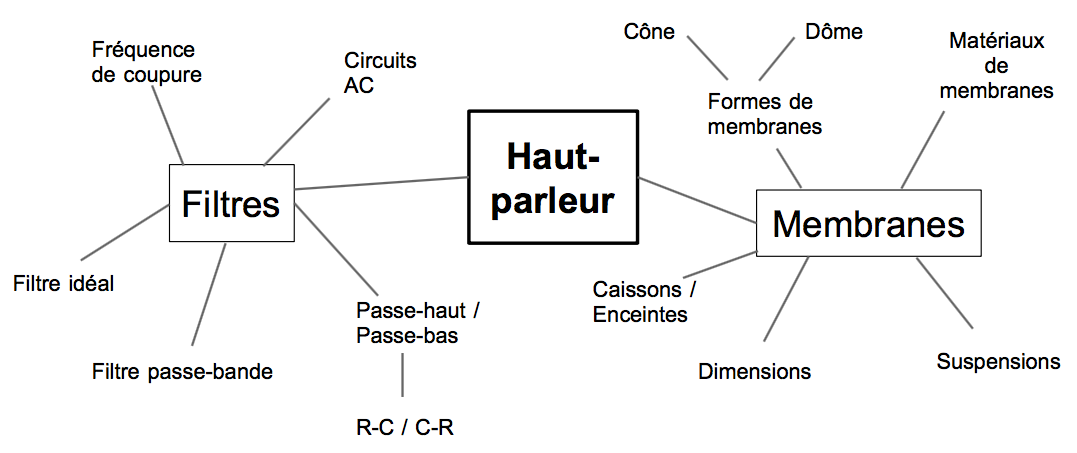
\includegraphics[scale=0.35]{img/Mots-clefs.png}
\end{center}
\caption{Schéma des mots-clés utilisés}
 \label{Schema mots-clefs}
\end{figure}


Nous nous en sommes servis pour rechercher dans l'index de livres, dans les moteurs de recherches pour trouver des brevets et sites fiables. Aussi bien en français qu'en anglais. Cette liste était régulièrement modifiée au cours de nos lectures. Pour la membrane, nous avons principalement récolté des brevets et des sites internet, tandis que pour les filtres, il s'agissait surtout de livres. 
Enfin, nous avons sélectionné parmi les nombreuses sources trouvées celles qui contenaient les informations nécessaires pour pouvoir rédiger un article sur les membranes et sur les filtres.
\newline

Ce travail nous a permis de nous rendre compte à quelle point la recherche documentaire est omniprésente dans tout travail scientifique pour acquérir les bases théoriques.
\newline

Vous trouverez dans les pages qui suivent des traces d'extraits qui nous ont été utiles (\ref{Trace 1}, \ref{Trace 2}, \ref{Trace 3}), ainsi qu'une liste des ressources bibliographiques.

\begin{figure}
\begin{center}
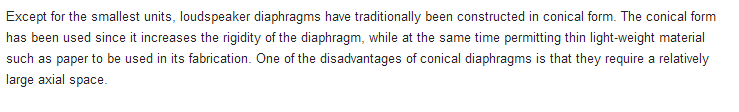
\includegraphics[scale=0.8]{img/Trace1-brevet US 3153463.png}
\end{center}
\caption{Trace 1 : extrait du brevet \textbf{ICI mettre ref vers brevet US3153463 de bibdesk}} 
 \label{Trace 1}
\end{figure}

\begin{figure}
\begin{center}
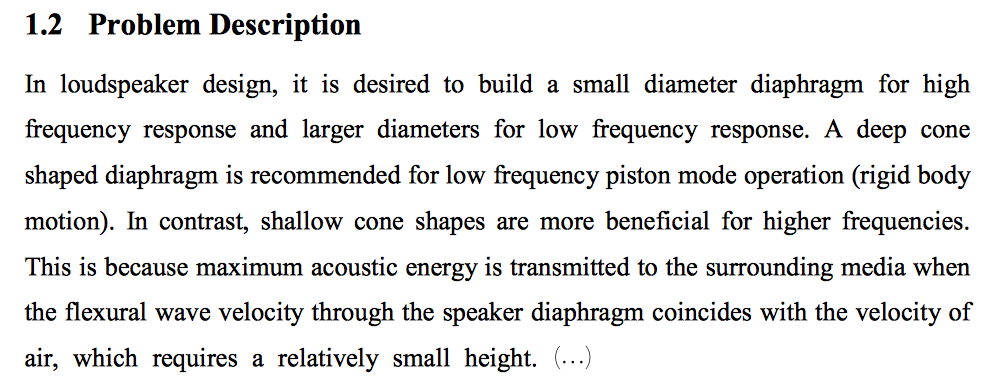
\includegraphics[scale=0.35]{img/Trace2-Miller.png}
\end{center}
\caption{Trace 2 : extrait du mémoire \textbf{ICI mettre ref vers mémoire de Ryan Miller de bibdesk}} 
 \label{Trace 2}
\end{figure}

\begin{figure}
\begin{center}
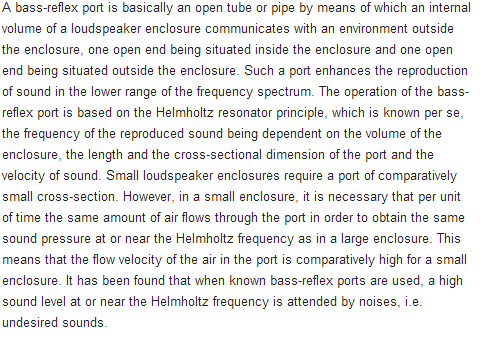
\includegraphics{img/Trace 3-US 1961149 A.png}
\end{center}
\caption{Trace 3 : extrait du brevet \textbf{ICI mettre ref vers brevet US1961149 A de bibdesk}} 
 \label{Trace 3}
\end{figure}



\

\

 
 
 
 
 




\chapter{Planning de travail}
\label{annexe:planning}

Lors des premières semaines du projet, nous avons établi un planning de travail (voir figure~\ref{fig:plan}), celui-ci a été construit de manière logique, en partant des idées les plus larges et en allant vers les tâches les plus concrètes. On voit très bien l'évolution en escalier au fil des semaines.

\begin{figure}	
\begin{center}
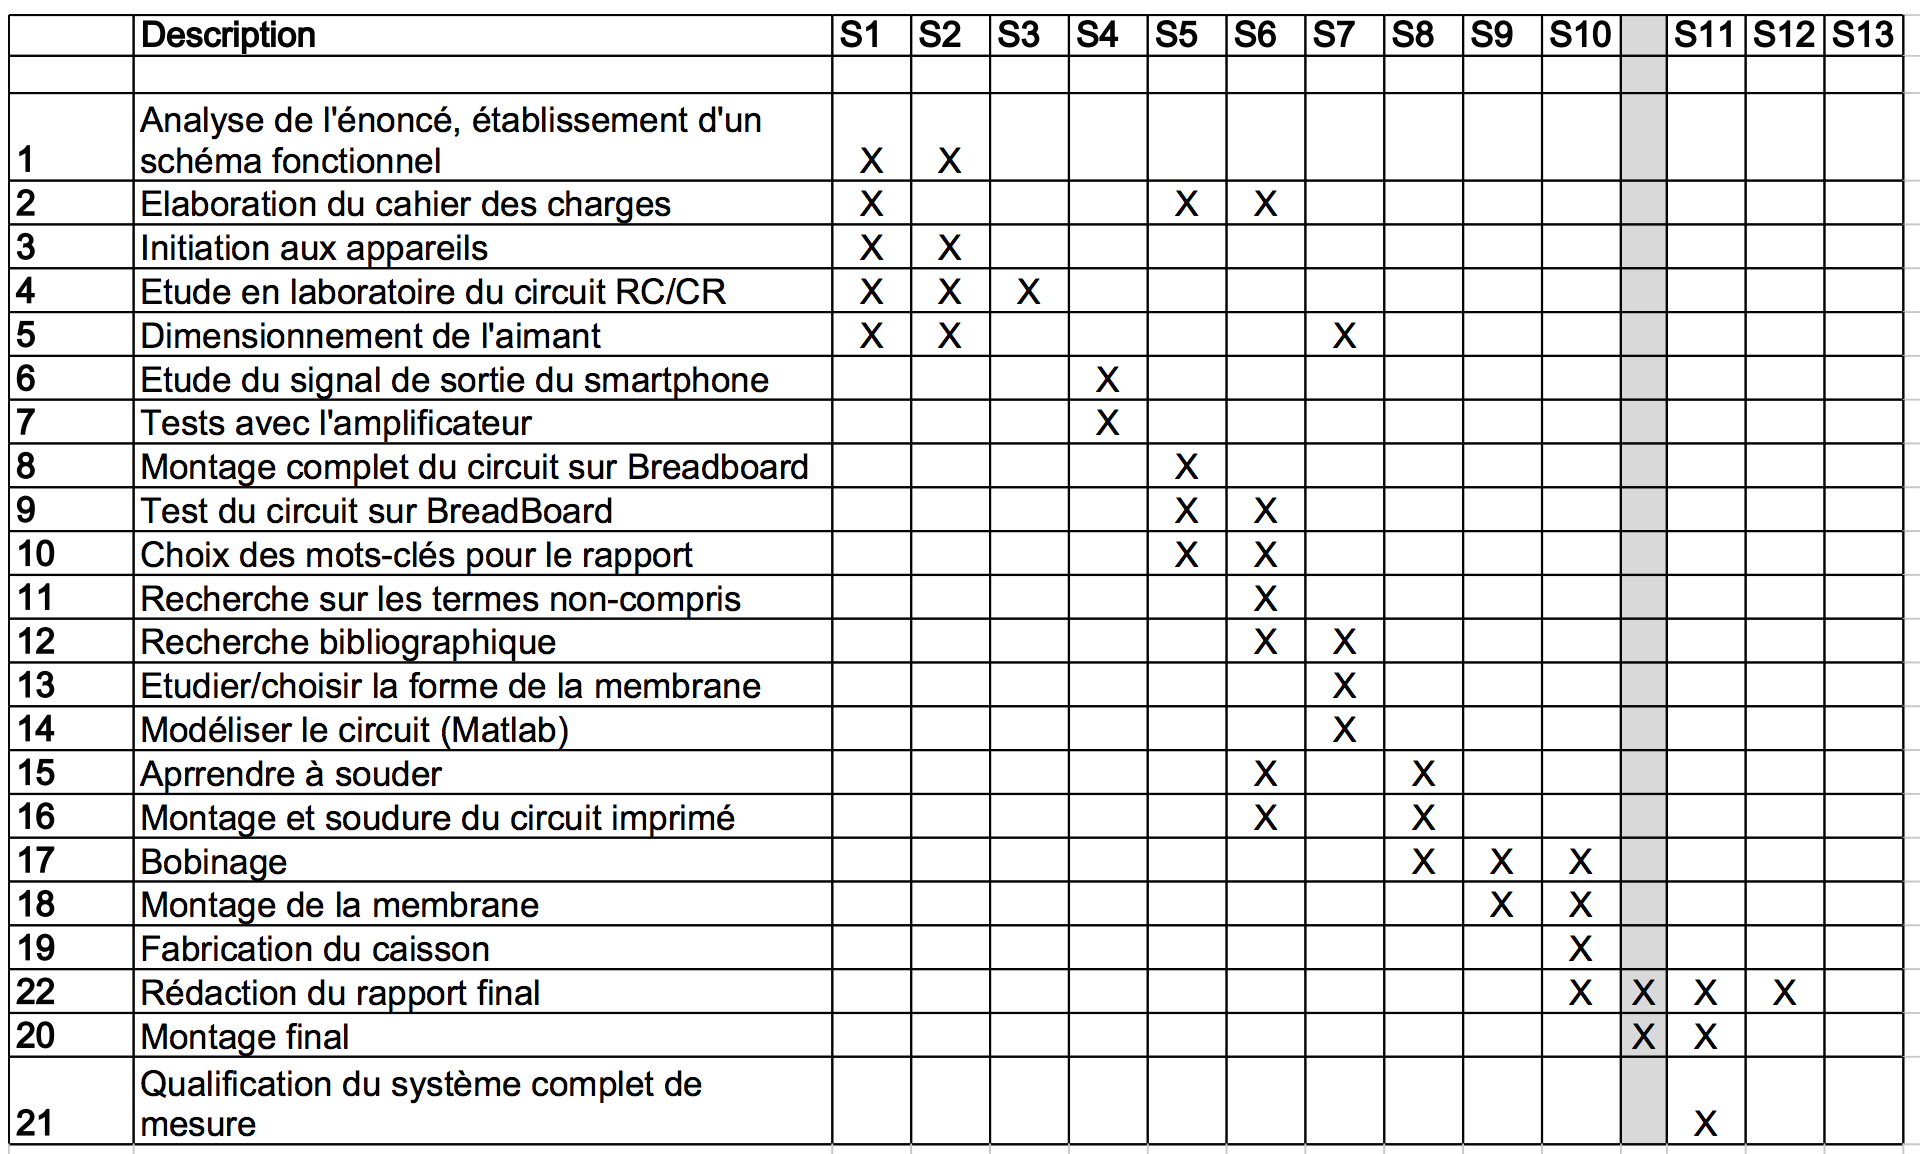
\includegraphics[width=\textwidth]{img/planning} 
\end{center}
\caption{Planning de travail}		
\label{fig:plan}		
\end{figure}

Tout d'abord, il nous a fallu analyser l'énoncé afin de créer un cahier des charges qui correspondait au mieux à ce qui nous était demandé et aux contraintes qui nous étaient imposées. 
En parallèle, au laboratoire, nous avons appris à utiliser les appareils de mesures et nos premières études se sont portées sur le fonctionnement des circuits CR/RC.

Ensuite, nous avons pu entrer dans le vif du sujet avec le dimensionnement de l'électroaimant, l'étude du signal de sortie du smartphone et le montage de circuit sur breadboard.

Après divers tests, nous avons appris à souder afin de monter le circuit sur la PCB. En parallèle, nous avons commencé la recherche documentaire, point essentiel à la compréhension de notre système.

A l'approche des vacances de Pâques, ils nous a fallu effectuer les bobinages ainsi que réaliser les caissons et les membranes pour notre haut-parleur. Nous avons à ce moment-là pu déjà effectuer les premiers tests sur le système complet.

Enfin, les derniers points qui restaient à aborder étaient la rédaction du rapport final, le montage final de notre haut-parleur et la qualification du système de mesure complet de celui-ci.


\chapter{Mesures effectuées}

\chapter{Codes MATLAB}

\section{Implémentations des 3 méthodes}

Les codes ci-dessous sont des implémentations des trois méthodes
d'identification linéaire.
Elles prennent en entrée les abcisses et ordonnées de mesures
et renvoient les coefficients de la droite trouvée.

Les trois implémentations s'exécutent en $O(n)$ et donnent le même résultat
à des erreurs de troncage près.

\lstset{
    language=Octave,
    basicstyle=\footnotesize,
    %title=\lstname,
    frame=single,
    numbers=left,
    breaklines=true,
}

\subsection{Méthode 1}
\lstinputlisting{code/approx_lin1.m}

\subsection{Méthode 2}
\lstinputlisting{code/approx_lin2.m}

\subsection{Méthode 3}
\lstinputlisting{code/approx_lin3.m}


\printbibliography[heading=bibintoc]

\end{document}
